In this section, numerical results of the proposed framework for the illustrative example in \sref{illustrative-example} are reported. All the experiments are implemented in MATLAB R2012a \cite{matlab} and conducted in \hostOS\ running on \hostHardware.

The channel length $\Leff$ is assumed to deviate by $5\%$ from the nominal value of $45$ nm where the global and local variations are equally weighted \cite{juan2011, juan2012}. Correlation matrices are computed according to \eref{correlation-matrix}, in which the correlation length $\corrLength$ is half the size of the die. In the model order reduction technique (see \sref{ie-uncertain-parameters}) the threshold parameter $\Lth$ is set to $0.99$ preserving $99\%$ of the variance of the data. Dynamic power profiles involved in the experiments are based on simulations of randomly generated applications defined as task graphs.\footnote{The task graphs of the applications, floorplans of the platforms, configuration of HotSpot, which is used for construction of the thermal RC circuits, are available online at \cite{sources}.} The floorplans of the platforms are constructed in such a way that the processing elements are placed in symmetric grids, as it is the case with, e.g., Alpha 21264 studied in \cite{juan2011}. Time steps of power and temperature traces are set to one millisecond, i.e., $\dt_i = 10^{-3}$s, $\forall i$ (see \sref{problem-formulation}). The reference leakage current $I_\leak(\Leff, \T)$ (see \sref{ie-power-model}) is scaled to account for about $40\%$ of the total power at high temperatures \cite{liu2007}. To assess the performance of our framework, we employ a Monte Carlo (MC) sampling technique. The MC approach solves \eref{fourier-original} at each iteration numerically using the Dormand-Prince method, which is based on the fourth- and fifth-order Runge-Kutta formulas \cite{press2007}. Based on theoretical estimations \cite{diaz-emparanza2002} of the accuracy of MC simulations, experience from the literature \cite{xiu2010, eldred2009, maitre2010, shen2009}, and our observations, we let the MC approach with $10^4$ samples be the etalon for the evaluation of our proposed technique.

The first set of experiments is aimed to identify the accuracy of our framework with respect to MC simulations.
At this point, it is important to note that the true distributions of temperature are unknown, and both the PC and MC approaches introduce errors.
These errors decrease as the order of PC expansions, $\pcorder$, and the number of MC samples, $\nsamples$, respectively, increase.
Therefore, instead of postulating that the MC technique with a certain number of samples is the ``universal truth'' that we should achieve, we shall vary both $\pcorder$ and $\nsamples$ and monitor the corresponding difference between the results produced by the two alternatives.

In order to make the comparison even more comprehensive, let us also inspect the effect of the correlation patterns between the local random variables $\lLeff_i(\o)$ (recall \sref{illustrative-example}).
Specifically, apart from $\pcorder$ and $\nsamples$, we shall change the balance between the two correlation kernels shown in \eref{correlation-function}, \ie, the squared-exponential $\fCorr_\SE$ and Ornstein-Uhlenbeck $\fCorr_\OU$ kernels, which is controlled by the weight parameter $\eta \in [0, 1]$.
In reality, of course, this parameter can take any value between zero and one.
Consequently, prior to any analysis, it should be determined based on the knowledge of the correlation structures typical for the fabrication process utilized.

The PC and MC methods are compared by means of three error metrics.
The first two are the normalized root mean square errors (\nrmses) of the expectation and variance of the computed temperature profiles.\footnote{In the context of \nrmses, we treat the MC results as the observed data and the PC results as the corresponding model predictions.}
The third metric is the mean of the \nrmses\ of the empirical \pdfs\ of temperature constructed at each time step for each processing element.
The metrics are denoted by $\eExp$, $\eVar$, and $\ePDF$, respectively.
$\eExp$ and $\eVar$ are easy to interpret, and they are based on the analytical formulae in \eref{pc-moments}.
$\ePDF$ is a strong indicator of the quality of the distributions estimated by our framework, and it is computed by sampling the constructed PC expansions.
In contrast with the MC approach, this sampling has a negligible overhead as we discussed in \sref{post-processing}.

The considered values for $\pcorder$, $\nsamples$, and $\eta$ are the sets $\{ n \}_{n = 1}^7$, $\{ 10^n \}_{n = 2}^5$, and $\{ 0, 0.5, 1 \}$, respectively.
The three cases of $\eta$ correspond to the total dominance of $\fCorr_\OU$ ($\eta = 0$), perfect balance between $\fCorr_\SE$ and $\fCorr_\OU$ ($\eta = 0.5$), and total dominance of $\fCorr_\SE$ ($\eta = 1$).
A comparison for a quad-core architecture with a dynamic power profile of $\nsteps = 10^2$ steps is given in \tref{accuracy-eta-0}, \tref{accuracy-eta-0-5}, and \tref{accuracy-eta-1}, which correspond to $\eta = 0$, $\eta = 0.5$, and $\eta = 1$, respectively.
Each table contains three subtables: one for $\eExp$ (the left most), one for $\eVar$ (in the middle), and one for $\ePDF$ (the right most), which gives nine subtables in total.
The columns of the tables that correspond to high values of $\nsamples$ can be used to assess the accuracy of the constructed PC expansions; likewise, the rows that correspond to high values of $\pcorder$ can be used to judge about the sufficiency of the number of MC samples.
One can immediately note that, in all the subtables, all the error metrics tend to decrease from the top left corners (low values of $\pcorder$ and $\nsamples$) to the bottom right corners (high values of $\pcorder$ and $\nsamples$), which suggests that the PC and MC methods converge.
There are a few outliers, associated with low PC orders and/or the random nature of sampling, \eg, $\eVar$ increases from 66.13 to 66.70 and $\ePDF$ from 1.59 to 1.62 when $\nsamples$ increases from $10^4$ and $10^5$ in \tref{accuracy-eta-0-5}; however, the aforementioned main trend is still clear.

For clarity of the discussions below, we shall primarily focus on one of the tables, namely, on the middle table, \tref{accuracy-eta-0-5}, as the case with $\eta = 0.5$ turned out to be the most challenging (explained in \sref{er-speed}).
The drawn conclusions will be generalized to the other two tables later on.

In this section, we focus on the computational speed of our framework.
First, we vary the number of processing elements $\nprocs$, which directly affects the dimensionality of the uncertain parameters $\vU(\o) \in \real^{\nprocs + 1}$ (recall \sref{illustrative-example}).
As before, we shall report the results obtained for various correlation weights $\eta$, which impacts the number of the independent variables $\vZ(\o) \in \real^\nvars$, preserved after the KL-based model order reduction procedure described in \sref{ie-uncertain-parameters} and \aref{karhunen-loeve}.

The results including the dimensionality of $\vZ(\o)$, $\nvars$, are given in \tref{speed-processing-elements} where the considered values for $\nprocs$ are $\{ 2^n \}_{n = 1}^5$, and the number of time steps $\nsteps$ is set to $10^3$.
It can be seen that the correlation patters inherent to the fabrication process \cite{cheng2011} open a great possibility for model order reduction: $\nvars$ is observed to be at most 12 while the maximal number without reduction is 33 (one global variable and 32 local ones corresponding to the case with 32 processing elements).
One can also observe how this number changes with respect to $\eta$: on average, the $\fCorr_\OU$ kernel ($\eta = 0$) requires the fewest number of variables while the mixture of $\fCorr_\SE$ and $\fCorr_\OU$ ($\eta = 0.5$) requires the most.\footnote{The results in \sref{er-accuracy} correspond to the case with $\nprocs = 4$; therefore, $\nvars$ is two, five, and five for \tref{accuracy-eta-0}, \tref{accuracy-eta-0-5}, and \tref{accuracy-eta-1}, respectively.}
It means that, in the latter case, more variables should be preserved in order to retain 99\% of the variance of the data; hence, the case with $\eta = 0.5$ is the most demanding in terms of complexity (see \sref{computational-challenges}).

Another observation, found in \tref{speed-processing-elements}, is the low slope of the execution time of the MC technique, which illustrates the well-known fact that the workload per one MC sample is independent of the number of stochastic dimensions \cite{maitre2010}.
On the other hand, the rows with $\nvars > 10$ hint at the curse of dimensionality possessed by PC expansions, which was discussed in \sref{computational-challenges}.
However, even in high dimensions, the proposed framework significantly outperforms MC sampling. For instance, in order to analyze a power profile with $10^3$ steps of a system with 32 cores, the MC approach requires more than 40 hours whereas the proposed framework takes less than two minutes (the case with $\eta = 0.5$).

Finally, we investigate the scaling properties of the proposed framework with respect to the duration of the considered time spans, which is directly proportional to the number of steps $\nsteps$ in the power and temperature profiles.
The results for a quad-core architecture are given in \tref{speed-time-spans}.
Due to the long execution times demonstrated by the MC approach, its statistics for high values of $\nsteps$ are extrapolated based on a smaller number of samples, \ie, $\nsamples \ll 10^4$.
As it was noted before regarding the results in \tref{speed-processing-elements}, we observe the dependency of the PC expansions on the dimensionality of $\vZ(\o)$, $\nvars$, which is two for $\eta = 0$ and five for the other two values of $\eta$ (see \tref{speed-processing-elements} for $\nprocs = 4$).
It can be seen in \tref{speed-time-spans} that the computational times of both methods grow linearly with $\nsteps$, which is expected.
However, the proposed framework shows a vastly superior performance being five orders of magnitude faster than MC sampling.

\begin{figure}[b]
  \vspace{-1.5em}
  \centering
  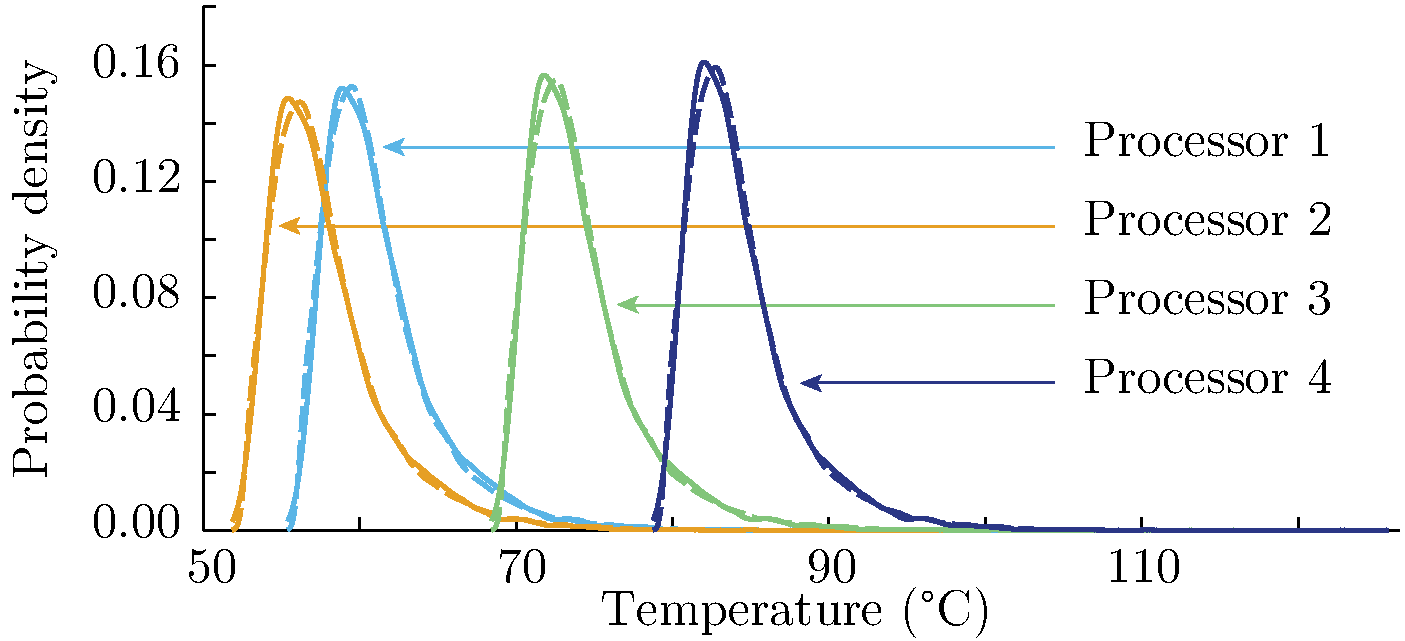
\includegraphics[width=1\ColumnWidth]{include/assets/experimental-results-pdf.pdf}
  \vspace{-2.0em}
  \caption{Probability density functions computed at time 50$\,\text{ms}$ using the proposed framework (the dashed lines) and MC sampling (the solid lines).}
  \flabel{experimental-results-pdf}
\end{figure}

First, we concentrate on the accuracy of our technique and, thus, pay particular attention the columns of \tref{accuracy-eta-0-5} corresponding to high values of $\nsamples$.
It can be seen that the error of the expected value, $\eExp$, is small even for $\pcorder = 1$: it is bounded by 0.6\% (see $\eExp$ for $\pcorder \geq 1$ and $\nsamples \geq 10^4$).

The error of the second central moment, $\eVar$, starts from 66.7\% for the first-order PC expansions and drops significantly to 5.71\% and below for the fourth order and higher (see $\eVar$ for $\pcorder \geq 4$ and $\nsamples = 10^5$).
It should be noted, however, that, for a fixed $\pcorder \geq 4$, $\eVar$ exhibits a considerable decrease even when $\nsamples$ transitions from $10^4$ to $10^5$.
The rate of this decrease suggests that $\nsamples = 10^4$ is not sufficient to reach the same accuracy as the one delivered by the proposed framework, and $\nsamples = 10^5$ might not be either.

The results of the third metric, $\ePDF$, allow us to conclude that the \pdfs\ computed by the third-order (and higher) PC expansions closely follow those estimated by the MC technique with large numbers of samples, namely, the observed difference in \tref{accuracy-eta-0-5} is bounded by 1.83\% (see $\ePDF$ for $\pcorder \geq 3$ and $\nsamples \geq 10^4$).
To give a better appreciation of the proximity of the two methods, \fref{experimental-results-pdf} displays the \pdfs\ computed using our framework for time moment 50~ms with $\pcorder = 4$ (the dashed lines) along with those calculated by the MC approach with $\nsamples = 10^4$ (the solid lines).
It can be seen that the \pdfs\ tightly match each other.
Note that this example captures one particular time moment, and such curves are readily available for all the other steps of the considered time span.

Now we take a closer look at the convergence of the MC-based technique.
With this in mind, we focus on the rows of \tref{accuracy-eta-0-5} that correspond to PC expansions of high orders.
Similar to the previous observations, even for low values of $\nsamples$, the error of the expected values estimated by MC sampling is relatively small, namely, bounded by 1.19\% (see $\eExp$ for $\pcorder \geq 4$ and $\nsamples = 10^2$).
Meanwhile, the case with $\nsamples = 10^2$ has a high error rate in terms of $\eVar$ and $\ePDF$: it is above 38\% for variance and almost 3.5\% for \pdfs\ (see $\eVar$ and $\ePDF$ for $\pcorder = 7$ and $\nsamples = 10^2$).
The results with $\nsamples = 10^3$ are reasonably more accurate; however, this trend is compromised by \tref{accuracy-eta-1}: $10^3$ samples leave an error of more than 7\% for variance (see $\eVar$ for $\pcorder \geq 4$ and $\nsamples = 10^3$).

The aforementioned conclusions, based on \tref{accuracy-eta-0-5} ($\eta = 0.5$), are directly applicable to \tref{accuracy-eta-0} ($\eta = 0$) and \tref{accuracy-eta-1} ($\eta = 1$).
The only difference is that the average error rates are lower when either of the two correlation kernels dominates.
In particular, according to $\eVar$, the case with $\eta = 1$, which corresponds to $\fCorr_\SE$, stands out to be the least error prone.

Guided by the observations in this subsection, we conclude that our framework delivers accurate results starting from $\pcorder = 4$.
The MC estimates, on the other hand, can be considered as sufficiently reliable starting from $\nsamples = 10^4$.
The last conclusion, however, is biased in favor of the MC technique since, as we noted earlier, there is evidence that $10^4$ samples might still not be enough.

The first set of experiments is aimed to identify the accuracy of our framework and, consequently, to find a reasonable value of the polynomial order $\pcorder$ (see \sref{polynomial-chaos}). To this end, three accuracy metrics have been chosen. The first two are the normalized root mean square errors (NRMSE) of expectation and variance of the resulting temperature traces. The third metric is the mean of NRMSEs of empirical probability density functions (PDFs) constructed at each time step for each processing element. The comparison for a quad-core architecture with a dynamic power profile of $\steps = 10^2$ steps is given in \fref{accuracy}, where $\pcorder$ is swept from $1$ to $5$. It can be seen that deviations of the expected value is small even for $\pcorder = 1$ and is bounded by $0.11\%$. The NRMSE of variance starts from $36\%$ for the first-order PC expansion and drops significantly to less than $2\%$ for the third-order PC. The result of the third error estimate, the NRMSE of PDFs, is of a particular importance since it allows us to conclude that the PDFs computed by the fourth-order (and higher) PC expansions are closely following those of the MC technique with a large number of samples. Guided by the above observations, we fix the polynomial order $\pcorder$ to four for the rest of the experiments and state that the error of our technique is bounded by less than $0.2\%$ for expectation and less than $2\%$ for variance and PDFs.

In this section, we focus on the computational speed of our framework.
First, we vary the number of processing elements $\nprocs$, which directly affects the dimensionality of the uncertain parameters $\vU(\o) \in \real^{\nprocs + 1}$ (recall \sref{illustrative-example}).
As before, we shall report the results obtained for various correlation weights $\eta$, which impacts the number of the independent variables $\vZ(\o) \in \real^\nvars$, preserved after the KL-based model order reduction procedure described in \sref{ie-uncertain-parameters} and \aref{karhunen-loeve}.

The results including the dimensionality of $\vZ(\o)$, $\nvars$, are given in \tref{speed-processing-elements} where the considered values for $\nprocs$ are $\{ 2^n \}_{n = 1}^5$, and the number of time steps $\nsteps$ is set to $10^3$.
It can be seen that the correlation patters inherent to the fabrication process \cite{cheng2011} open a great possibility for model order reduction: $\nvars$ is observed to be at most 12 while the maximal number without reduction is 33 (one global variable and 32 local ones corresponding to the case with 32 processing elements).
One can also observe how this number changes with respect to $\eta$: on average, the $\fCorr_\OU$ kernel ($\eta = 0$) requires the fewest number of variables while the mixture of $\fCorr_\SE$ and $\fCorr_\OU$ ($\eta = 0.5$) requires the most.\footnote{The results in \sref{er-accuracy} correspond to the case with $\nprocs = 4$; therefore, $\nvars$ is two, five, and five for \tref{accuracy-eta-0}, \tref{accuracy-eta-0-5}, and \tref{accuracy-eta-1}, respectively.}
It means that, in the latter case, more variables should be preserved in order to retain 99\% of the variance of the data; hence, the case with $\eta = 0.5$ is the most demanding in terms of complexity (see \sref{computational-challenges}).

Another observation, found in \tref{speed-processing-elements}, is the low slope of the execution time of the MC technique, which illustrates the well-known fact that the workload per one MC sample is independent of the number of stochastic dimensions \cite{maitre2010}.
On the other hand, the rows with $\nvars > 10$ hint at the curse of dimensionality possessed by PC expansions, which was discussed in \sref{computational-challenges}.
However, even in high dimensions, the proposed framework significantly outperforms MC sampling. For instance, in order to analyze a power profile with $10^3$ steps of a system with 32 cores, the MC approach requires more than 40 hours whereas the proposed framework takes less than two minutes (the case with $\eta = 0.5$).

Finally, we investigate the scaling properties of the proposed framework with respect to the duration of the considered time spans, which is directly proportional to the number of steps $\nsteps$ in the power and temperature profiles.
The results for a quad-core architecture are given in \tref{speed-time-spans}.
Due to the long execution times demonstrated by the MC approach, its statistics for high values of $\nsteps$ are extrapolated based on a smaller number of samples, \ie, $\nsamples \ll 10^4$.
As it was noted before regarding the results in \tref{speed-processing-elements}, we observe the dependency of the PC expansions on the dimensionality of $\vZ(\o)$, $\nvars$, which is two for $\eta = 0$ and five for the other two values of $\eta$ (see \tref{speed-processing-elements} for $\nprocs = 4$).
It can be seen in \tref{speed-time-spans} that the computational times of both methods grow linearly with $\nsteps$, which is expected.
However, the proposed framework shows a vastly superior performance being five orders of magnitude faster than MC sampling.

Now, we focus on the computational speed. First, we vary the number of processing elements $\cores$ and, consequently, the number of \rvs\ $\vars$. In these experiments, the number of time steps $\steps$ is constant and equal to $10^3$. The results are given in \tref{scaling-cores} along with the number of \rvs\ left after the PCA (see \sref{ie-uncertain-parameters}). It can be seen that the typical symmetric placement and natural radial structure of correlations \cite{cheng2011} open a great possibility for model order reduction. One can also observe a low slope of the execution time of the MC technique, which demonstrates the well-known fact that the workload per one MC sample is independent of the number of \rvs\  \cite{maitre2010}. At the same time, the PC demonstrates a polynomial growth \cite{heiss2008} of the computational time. However, even in high dimensions, the proposed framework significantly outperforms the MC sampling. For instance, to quantify a power profile with $10^3$ steps of a multiprocessor system with $32$ cores, the MC approach requires more than $40$ hours whereas the proposed framework takes less than 10 seconds.

Finally, we investigate the scaling properties of the proposed framework with respect to the number of time steps $\steps$ in the input power profile, which is directly proportional to the considered time span. The results for a quad-core architecture are given in \tref{scaling-steps}. Due to the long execution time demonstrated by the MC approach, its computational times for high values of $\steps$ are extrapolated based on a few samples. It can be seen that both methods scale linearly. However, the proposed framework shows a vastly superior performance.
